
% Infrastruktur
% Implementierung
	% Ordnerstruktur
	% Patterns
		% PageObject
		% PageFactory
	% Architektur
		% TestRunners
	% Testbeschreibung

\chapter{Umsetzung}
\label{sec:umsetzung}

\section{Prozess}
Der Prozess wurde equivalent aufgesetzt, wie es im \cref{sec:konzept:prozess} \nameref{sec:konzept:prozess} beschrieben wurde.

\begin{figure}[H]
	\centering
	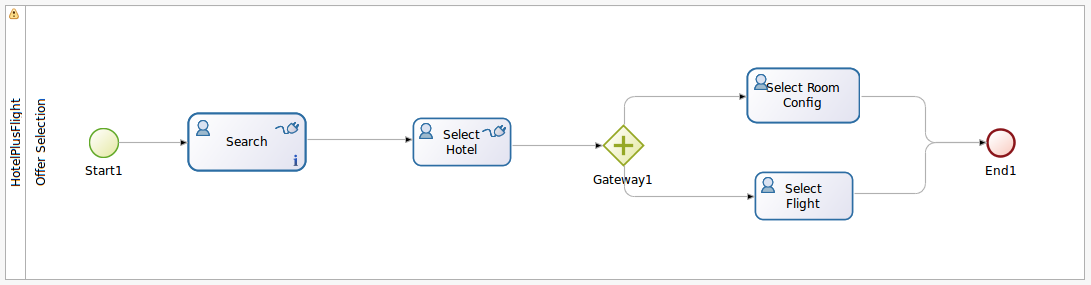
\includegraphics[width=1\textwidth]{images/umsetzung-prozess.png}
	\caption{Prozess im Bonita BPM}
	\label{fig:umsetzung:prozess}
\end{figure}
Das Icon oben links im Task signalisiert, dass es sich dabei um einen Human Task handelt und eine Benutzerinteraktion erforderlich ist. Das Bild oben rechts im Task zeigt an, dass es einen Connector auf dem Task gibt.

\section{Business Data Models und Pool Variables}
Als \glspl{bdm} wurden folgende Modelle definiert:
\begin{table}[H] 
	\caption{Business Data Models}
	\centering
	\label{sec:umsetzung:bdm:bdm}
	
	\begin{tabular}{ | l | l | c | } 
		\hline
		\textbf{Name} & \textbf{Type} & \textbf{Multiple} \\ \hline 
		\multicolumn{3}{|c|}{\textbf{HotelPlusFlightSearch}} \\ \hline 
		destination & string & \\ \hline
		departure & string & \\ \hline
		adults & integer & \\ \hline
		fromDate & date & \\ \hline
		toDate & date & \\ \hline
		id & string & \\ \hline
		\multicolumn{3}{|c|}{\textbf{HotelPlusFlightResults}} \\ \hline 
		hotels & HotelPlusFlightResultHotel & x \\ \hline
		\multicolumn{3}{|c|}{\textbf{HotelPlusFlightResultHotel}} \\ \hline 
		name & string & \\ \hline
		price & string & \\ \hline
		image & string & \\ \hline
		roomConfigs & HotelPlusFlightRoomConfig & x \\ \hline
		flights & HotelPlusFlightFlightResult & x \\ \hline
		id & string & \\ \hline
		\multicolumn{3}{|c|}{\textbf{HotelPlusFlightRoomConfig}} \\ \hline 
		roomType & string & \\ \hline
		mealType & string & \\ \hline
		id & string & \\ \hline
		\multicolumn{3}{|c|}{\textbf{HotelPlusFlightFlightResult}} \\ \hline 
		airline & string & \\ \hline
		fromAirport & string & \\ \hline
		toAirport & string & \\ \hline
		flight1FromTime & string & \\ \hline
		flight1ToTime & string & \\ \hline
		flight2FromTime & string & \\ \hline
		flight2ToTime & string & \\ \hline
		id & string & \\ \hline
	\end{tabular} 
\end{table}

Auf der Poolebene wurde für jedes \gls{bdm} eine Pool Variable erstellt. Der Name der Variable entspricht dem \gls{bdm}, beginnt jedoch mit einem kleinen Buchstaben.
\begin{table}[H] 
	\caption{Pool Variables}
	\centering
	\label{sec:umsetzung:bdm:poolvariable}
	
	\begin{tabular}{ | l | l | c | } 
		\hline
		\textbf{Name} & \textbf{BDM} \\ \hline 
		hotelPlusFlightSearch & HotelPlusFlightSearch \\ \hline
		hotelPlusFlightResults & HotelPlusFlightResults \\ \hline
		hotelPlusFlightResultHotel & HotelPlusFlightResultHotel \\ \hline
		hotelPlusFlightRoomConfig & HotelPlusFlightRoomConfig \\ \hline
	 	hotelPlusFlightFlightResult & HotelPlusFlightFlightResult \\ \hline
	\end{tabular} 
\end{table}
\section{Forms}
Die Formulare wurden bereits für die Mockups im \cref{sec:konzept:mockups} \nameref{sec:konzept:mockups} erstellt und konnten gleich wiederverwendet werden. Deshalb wird hier auf eine erneute Auflistung verzichtet.

\section{Connectors}
Nachfolgend werden die Definitionen und Implementationen der Connectors beschrieben. Zusätzlich werden für deren Ausführung weitere Abhängigkeiten benötigt, welche in Bonita BPM definiert werden müssen.

\subsection{Abhängigkeiten}
Für die Ausführung der Connectoren können in Bonita BPM weitere Libraries hinterlegt werden. Für dieses Projekt wurden zusätzlich zwei Abhängigkeiten definiert. Zum Einen Gson\footcite{Gson_2016-06-12}, für die Bearbeitung von JSON, und zum anderem Handy URI Templates\footcite{HandyUriTempaltes_2016-06-12}, für die Verarbeitung von URI Templates gemäss RFC 6570\footcite{RFC_6570_-_URI_Template_2016-06-21}.

\subsection{Definitions}
Es wurden vier Definitionen erstellt. Für jeden Task einer.

\begin{table}[H] 
	\caption{Connector Definitions}
	\centering
	\label{sec:umsetzung:connectors:definitions}
	
	\begin{tabular}{ | l | l | l | l | } 
		\hline
		\textbf{Name} & \textbf{Input} & \textbf{Wizard pages} & \textbf{Outputs} \\ \hline 
		H+FSearch & H+FSearch & & H+FResults \\ \hline
		H+FResultsHotelSelection & HotelPlusFlightResults & Results & H+FResultHotel \\ \hline
		H+FHotelConfiguration & H+FResultHotel & Hotel & H+FResults \\ \hline
		H+FFlightSelection & H+FResultHotel & Hotel & H+FFlightResult \\ \hline
	\end{tabular} 
\end{table}

\subsection{Implementations}

\section{Tasks}
Nachfolgend werden die Tasks im Prozess beschrieben. Diese bestehen aus einem Bezeichner und einem Connector. Zusätzlich müssen noch der Contract, das Formular sowie die Operations (siehe \cref{sec:analyse:bonita:forms} \nameref{sec:analyse:bonita:forms}) angegeben werden.

\subsection{Search}
Der Search Task muss ein Formular darstellen, damit der Benutzer seine Suchkriterien eingeben kann. Dazu wird der Connector HotelPlusFlugSearch hinterlegt und das Formular hotelPlusFlightSearchForm unter Connectors out definiert.

Folgender Contract und Operations mussten spezifiziert werden:
\begin{table}[H] 
	\caption{Search Task Contract}
	\centering
	
	\begin{tabular}{ | l | l | c | } 
		\hline
		\textbf{Name} & \textbf{Type} & \textbf{Multiple} \\ \hline 
		hotelPlusFlightSearchInput & complex & \\ \hline
		\hspace*{5mm}destination & text & \\ \hline
		\hspace*{5mm}departure & text & \\ \hline
		\hspace*{5mm}adults & integer & \\ \hline
		\hspace*{5mm}fromDate & date & \\ \hline
		\hspace*{5mm}toDate & date & \\ \hline
	\end{tabular} 
\end{table}
\begin{table}[H] 
	\caption{Search Task Operations}
	\centering
	
	\begin{tabular}{ | l | l | l | } 
		\hline
		\textbf{Business Data Model} & \textbf{Operation} & \textbf{Form Variable} \\ \hline 
		hotelPlusFlightSearch & setDestination & H+FSearchInput.destination \\ \hline
		hotelPlusFlightSearch & setDeparture & H+FSearchInput.departure \\ \hline
		hotelPlusFlightSearch & setAdults & H+FSearchInput.adults \\ \hline
		hotelPlusFlightSearch & setFromDate & H+FSearchInput.fromDate \\ \hline
		hotelPlusFlightSearch & setToDate & H+FSearchInput.toDate \\ \hline
	\end{tabular} 
\end{table}

\subsection{Select Hotel}
Der Select Hotel Task nimmt eine Liste von Hotels entgegen und speichert danach das selektierte ab. Dazu wird der Connector HotelPlusFlightResultsHotelSelection unter Connectors out und das Formular hotelPlusFlightHotelSelection hinterlegt.

Folgender Contract und Operations mussten spezifiziert werden:
\begin{table}[H] 
	\caption{Select Hotel Task Contract}
	\centering
	
	\begin{tabular}{ | l | l | c | } 
		\hline
		\textbf{Name} & \textbf{Type} & \textbf{Multiple} \\ \hline 
		hotelPlusFlightResultsInput & complex & \\ \hline
		\hspace*{5mm}hotels & complex & x \\ \hline
		\hspace*{10mm}name & text & \\ \hline
		\hspace*{10mm}price & text & \\ \hline
		\hspace*{10mm}image & text & \\ \hline
	\end{tabular} 
\end{table}
\begin{table}[H] 
	\caption{Select Hotel Task Operations}
	\centering
	
	\begin{tabular}{ | l | l | l | } 
		\hline
		\textbf{Business Data Model} & \textbf{Operation} & \textbf{Form Variable} \\ \hline 
		hotelPlusFlightSearch & setDestination & H+FSearchInput.destination \\ \hline
		hotelPlusFlightSearch & setDeparture & H+FSearchInput.departure \\ \hline
		hotelPlusFlightSearch & setAdults & H+FSearchInput.adults \\ \hline
		hotelPlusFlightSearch & setFromDate & H+FSearchInput.fromDate \\ \hline
		hotelPlusFlightSearch & setToDate & H+FSearchInput.toDate \\ \hline
	\end{tabular} 
\end{table}

\subsection{Select Room Config}
Beim Schritt Select Room Config wird das selektierte Hotel übergeben und der Benutzer kann eine Zimmerkonfiguration auswählen. Dafür ist das From hotelPlusFlightSelectRoomConfig und der Connector HotelPlusFlightHotelConfiguration (im Connector out) vorgesehen.

Folgender Contract und Operations mussten spezifiziert werden:
\begin{table}[H] 
	\caption{Select Room Config Task Contract}
	\centering
	
	\begin{tabular}{ | l | l | c | } 
		\hline
		\textbf{Name} & \textbf{Type} & \textbf{Multiple} \\ \hline 
		hotelPlusFlightRoomConfigsInput & complex & \\ \hline
		\hspace*{5mm}configs & complex & x \\ \hline
		\hspace*{10mm}RoomType & text & \\ \hline
		\hspace*{10mm}MealType & text & \\ \hline
		\hspace*{10mm}Price & text & \\ \hline
	\end{tabular} 
\end{table}
\begin{table}[H] 
	\caption{Select Room Config Task Operations}
	\centering
	
	\begin{tabular}{ | l | l | l | } 
		\hline
		\textbf{Business Data Model} & \textbf{Operation} & \textbf{Form Variable} \\ \hline 
		hotelPlusFlightRoomConfig & setConfig & H+FRoomConfigsInput.config \\ \hline
	\end{tabular} 
\end{table}

\subsection{Select Flight}
Beim letzten Task muss der User einen Flug auswählen. Dazu wird dem Task das gewählte Hotel übergeben. Definiert wurde das Formular hotelPlusFlightSelectFlight und der Connector out HotelPlusFlightFlightSelection.

Folgender Contract und Operations mussten spezifiziert werden:
\begin{table}[H] 
	\caption{Select Flight Task Contract}
	\centering
	
	\begin{tabular}{ | l | l | c | } 
		\hline
		\textbf{Name} & \textbf{Type} & \textbf{Multiple} \\ \hline 
		hotelPlusFlightFlightResultsInput & complex & \\ \hline
		\hspace*{5mm}flights & complex & x \\ \hline
		\hspace*{10mm}Airline & text & \\ \hline
		\hspace*{10mm}FromAirport & text & \\ \hline
		\hspace*{10mm}ToAirport & text & \\ \hline
		\hspace*{10mm}Flight1FromTime & text & \\ \hline
		\hspace*{10mm}Flight1ToTime & text & \\ \hline
		\hspace*{10mm}Flight2FromTime & text & \\ \hline
		\hspace*{10mm}Flight2ToTime & text & \\ \hline
	\end{tabular} 
\end{table}
\begin{table}[H] 
	\caption{Select Flight Task Operations}
	\centering
	
	\begin{tabular}{ | l | l | l | } 
		\hline
		\textbf{Business Data Model} & \textbf{Operation} & \textbf{Form Variable} \\ \hline 
		hotelPlusFlightFlightResult & setFlight & H+FFlightsInput.flight \\ \hline
	\end{tabular} 
\end{table}

\section{Probleme}
Es gab zwei Prolbeme, welche es verunmöglichten einen sauberen Prozess durchzuführen. Diese werden nachfolgend beschrieben.

\subsection{Rückgabewert der Connectors}
Der Connector HotelPlusFlight Search gibt ein HotelPlusFlightResults \gls{bdm} zurück. Dieses wird beim Connector Output in eine Pool Variable geschrieben. Dabei tritt folgender Fehler auf:
\begin{lstlisting}
java.lang.reflect.InvocationTargetException
com.thoughtworks.xstream.converters.ConversionException: com.travelwindow.model.HotelPlusFlightResults : com.travelwindow.model.HotelPlusFlightResults
---- Debugging information ----
message : com.travelwindow.model.HotelPlusFlightResults
cause-exception : com.thoughtworks.xstream.mapper.CannotResolveClassException
cause-message : com.travelwindow.model.HotelPlusFlightResults
class : java.util.HashMap
required-type : java.util.HashMap
converter-type : com.thoughtworks.xstream.converters.collections.MapConverter
path : /map/entry/com.travelwindow.model.HotelPlusFlightResults
line number : 5
version : null

com.thoughtworks.xstream.mapper.CannotResolveClassException: com.travelwindow.model.HotelPlusFlightResults
\end{lstlisting}
Bonita BPM unterstützt Groovy Scripts\footcite{Groovy_2016-06-25}, mit welcher man Daten verarbeiten kann. Es wurde versucht damit das Problem zu beheben.

Folgender Groovy Code wurde verwendet, um das Mapping für die HotelPlusFlightResults durchzuführen:
\begin{lstlisting}[language=Groovy,firstnumber=1]
import groovy.json.JsonBuilder
import com.travelwindow.model.HotelPlusFlightResults
import com.travelwindow.model.HotelPlusFlightResultHotel

def mappedData = new HotelPlusFlightResults()
for (hotel in hotelPlusFlightResults.getHotels()) {
	def tempHotel = new HotelPlusFlightResultHotel()
	tempHotel.name = comment.name
	tempHotel.image = comment.image
	tempHotel.price = comment.price
	mappedData.hotels.add(tempHotel)
}
return mappedData
\end{lstlisting}
Leider konnte der Fehler dadurch nicht behoben werden. Gemäss Bonitasoft sollte dies kein Problem darstellen. Recherchen in der Dokumentation des Programmes und Online im Forum des Herstellers gaben keine Abhilfe. Es wurden stattdessen Standartwerte auf den Pool Variablen definiert, damit der Prozess bis ans Ende durchgeführt werden kann.

\subsection{Input Parameter der Connectoren}
Das Aufsetzten der Formulare und die Konfiguration der Contract und Operations verlief problemlos. Jedoch gab es Probleme bei den Input Parametern der Connectoren. Bei der Ausführung des Prozesses erschien folgende Log Meldung:

\begin{lstlisting}[firstnumber=1]
SEVERE: THREAD_ID=119 | HOSTNAME=Slang-ThinkPad | TENANT_ID=1 | The work [ExecuteConnectorOfActivity: flowNodeInstanceId = 240003, connectorDefinitionName = HotelPlusFlighResultsHotelSelection] failed. The failure will be handled.
2016-06-25 15:07:57.211 +0200 org.bonitasoft.engine.execution.work.FailureHandlingBonitaWork org.bonitasoft.engine.log.technical.TechnicalLoggerSLF4JImpl log 
SEVERE: THREAD_ID=119 | HOSTNAME=Slang-ThinkPad | TENANT_ID=1 | org.bonitasoft.engine.persistence.SRetryableException : "Groovyx.persistence.PersistenceException: org.hibernate.PropertyValueException: not-null property references a null or transient value: com.travelwindow.model.HotelPlusFlightResultHotel._hotels_HOTELPLUSFLIGHTRESULTS_PIDBackref"
org.bonitasoft.engine.persistence.SRetryableException: javax.persistence.PersistenceException: org.hibernate.PropertyValueException: not-null property references a null or transient value: com.travelwindow.model.HotelPlusFlightResultHotel._hotels_HOTELPLUSFLIGHTRESULTS_PIDBackref
\end{lstlisting}

Der Fehler tritt nach dem Select Hotel Task auf, wenn der Connector HotelPlusFlightResultsHotelSelection aufgerufen wird. Ziel des Connectors ist es das gewählte Hotel aus der Liste der Resultate auszuwählen.

Der Fehler liegt gemäss der Logmeldung in dem Input Parameter, welcher an den Connector übergeben wird.
Unklar war, ob der Fehler in der Operations des Formulares liegt, oder am Connector selber.

\subsubsection{Script zum Abspeichern der Formularwerte}
Mit Groovy\footcite{Groovy_2016-06-25} kann man die Formularwerte bearbeitet, welche von den Formularen zurückgeliefert werden.
Es wurde folgendes Script definiert, um den Wert des Formulars in ein \gls{bdm} zu überführen, damit Bonita BPM diesen weiterverwenden kann. Dies wurde durchgeführt, in der Vermutung, dass eventuell der Fehler innerhalb der Operations des Formulars liegt.
\begin{lstlisting}[language=Groovy,firstnumber=1]
def hotels = new java.util.ArrayList()
hotelPlusFlightResultsInput.hotels.each{
	hotels.add({ currentHotelInput ->
		def tempHotel = new com.travelwindow.model.HotelPlusFlightResultHotel()
		tempHotel.name = currentHotelInput.name
		tempHotel.price = currentHotelInput.price
		tempHotel.image = currentHotelInput.image
		return tempHotel
	}(it))
}
def results = new com.travelwindow.model.HotelPlusFlightResults()
results.setHotels(hotels)
return results
\end{lstlisting}

Der Fehler blieb jedoch der selbe.

\subsubsection{Standartwerte definieren}
Es wurde eine neue Pool Variable vom Typ  HotelPlusFlightResults erstellt, welche mit fix vorgegebenen Werten befüllt wurde. Dies sollte ausschliessen, dass das Problem im Formular liegt. Auch dies wurde mit einem Groovy Script bewerkstelligt.

\begin{lstlisting}[language=Groovy,firstnumber=1]
def hotel1 = new com.travelwindow.model.HotelPlusFlightResultHotel()
hotel1.name = "Radisson Blu Hotel Berlin"
hotel1.image = "https://t-static.net/pictures/Hotel/Hotelbeds/9274/009274a_hb_ba_003.jpg?width=240&height=180&scale=both&mode=crop"
hotel1.price = "482 CHF"


def hotel2 = new com.travelwindow.model.HotelPlusFlightResultHotel()
hotel2.name = "NH Berlin Mitte"
hotel2.image = "https://t-static.net/pictures/Hotel/Hotelbeds/8819/008819a_hb_ba_008.jpg?width=240&height=180&scale=both&mode=crop"
hotel2.price = "403 CHF"

def hotel3 = new com.travelwindow.model.HotelPlusFlightResultHotel()
hotel3.name = "Wyndham Berlin Excelsior"
hotel3.image = "https://t-static.net/pictures/Hotel/Hotelbeds/5847/005847a_hb_l_010.jpg?width=240&height=180&scale=both&mode=crop"
hotel3.price = "350 CHF"

def hotels = new java.util.ArrayList()
hotels.add(hotel1)
hotels.add(hotel2)
hotels.add(hotel3)

def results = new com.travelwindow.model.HotelPlusFlightResults()
results.setHotels(hotels)
return results
\end{lstlisting}

Der Fehler blieb weiterhin bestehen.

\subsubsection{Input Parameter des Connectors entfernen}
Nun wurde versucht den Input Parameter des HotelPlusFlightResultsHotelSelection auf der Connector Definition zu entfernen.

Danach musste der Out Connector auf dem Select Hotel Task noch angepasst werden, um der Änderung in der Definition zu entsprechen.

Jedoch blieb der Fehler der selbe.

\subsubsection{Connector entfernen}
\label{sec:umsetzung:problem:removeconnector}
Als letzte Möglichkeit wurde der Connector aus dem Task Select Hotel entfernt. Damit verschwand auch der Fehler und der Prozess konnte durchgeführt werden.

\subsubsection{Konsequenz}
Es wurde noch weiter versucht dieses Problem zu beheben. Jedoch ohne Erfolg. Auch im Forum des Herstellers gab es keine Abhilfe. Deshalb mussten die Connectors auf den Tasks Select Hotel, Select Room Config und Select Flight entfernt werden, um zumindest in der Lage zu sein, den Prozess bis ans Ende durchzuführen. Deshalb wurde für alle Formulare Standartwerte Definiert, damit der Prozess bis ans Ende getestet werden kann.

Ein Beispiel für Standartwerte des Flugselections-Formular:
\begin{lstlisting}[language=json,firstnumber=1]
{
  "hotelPlusFlightFlightResultsInput" : {
    "flights" : [
        { "Airline": "LH", "FromAirport": "ZRH", "ToAirport": "TXL", "Flight1FromTime": "20.10.2016 20:15", 
        "Flight1ToTime": "20.10.2016 22:15", "Flight2FromTime": "22.10.2016 12:25", "Flight2ToTime": "22.10.2016 14:35"},
        { "Airline": "LX", "FromAirport": "ZRH", "ToAirport": "TXL", "Flight1FromTime": "20.10.2016 16:00", 
        "Flight1ToTime": "20.10.2016 18:05", "Flight2FromTime": "22.10.2016 20:45", "Flight2ToTime": "22.10.2016 22:40"},
        { "Airline": "LX", "FromAirport": "ZRH", "ToAirport": "TXL", "Flight1FromTime": "20.10.2016 06:30", 
        "Flight1ToTime": "20.10.2016 08:35", "Flight2FromTime": "22.10.2016 16:00", "Flight2ToTime": "22.10.2016 18:00"}
    ]
  }
}
\end{lstlisting}
